\chapter{Images}


Contrary to the classical notion of image employed in image processing, a medical image corresponds to the acquisition of an 3D (anatomical) volume\footnote{We consider here only 3D scalar images. Generalization to other dimensions and other modalities can be trivially deduced from the 3D case.}. The volume is discretized by first defining a virtual grid in the volume to acquire. Each element of the grid, called voxel for \textit{volume element}, receive a value computed from the integration of a given signal on an elementary volume centered on the considered voxel. The grid and its associated values are then stored into a 3D array.
\\

Considering the 3D array to represent a volume has been norm the for long. However, over the years, research studies proved that adding geometrical and anatomical information allowed to greatly improve computations. For instance, the information relative to the voxel size -- distance between two adjacent voxels -- has been proved to be very useful if not essential. Recent acquisition devices provide more geometrical (or positioning) information, such as image origin and image orientation, that may really help any process on images (see Figure~\ref{fig:position}).
\\
As a consequence, for each image, we have two different coordinate systems. First, the image coordinate system allow to access to the voxel value using classical indexes (\textit{e.g.} $I(i,j,k)$). Second, the world coordinate system position each voxel according to a coordinate system shared by all images. These coordinate systems and the projection from one system to the other one are presented in section~\ref{sec:image:systems}.
\\

Most if discretization implies a lost of information. The notion of image interpolation, well know in the image processing community, tries to recover the information lost during this discretization process. We present briefly in section~\ref{sec:image:interpolation} some interpolation algorithms used in medical imaging.

%
\begin{figure}[!htbp]
\centering
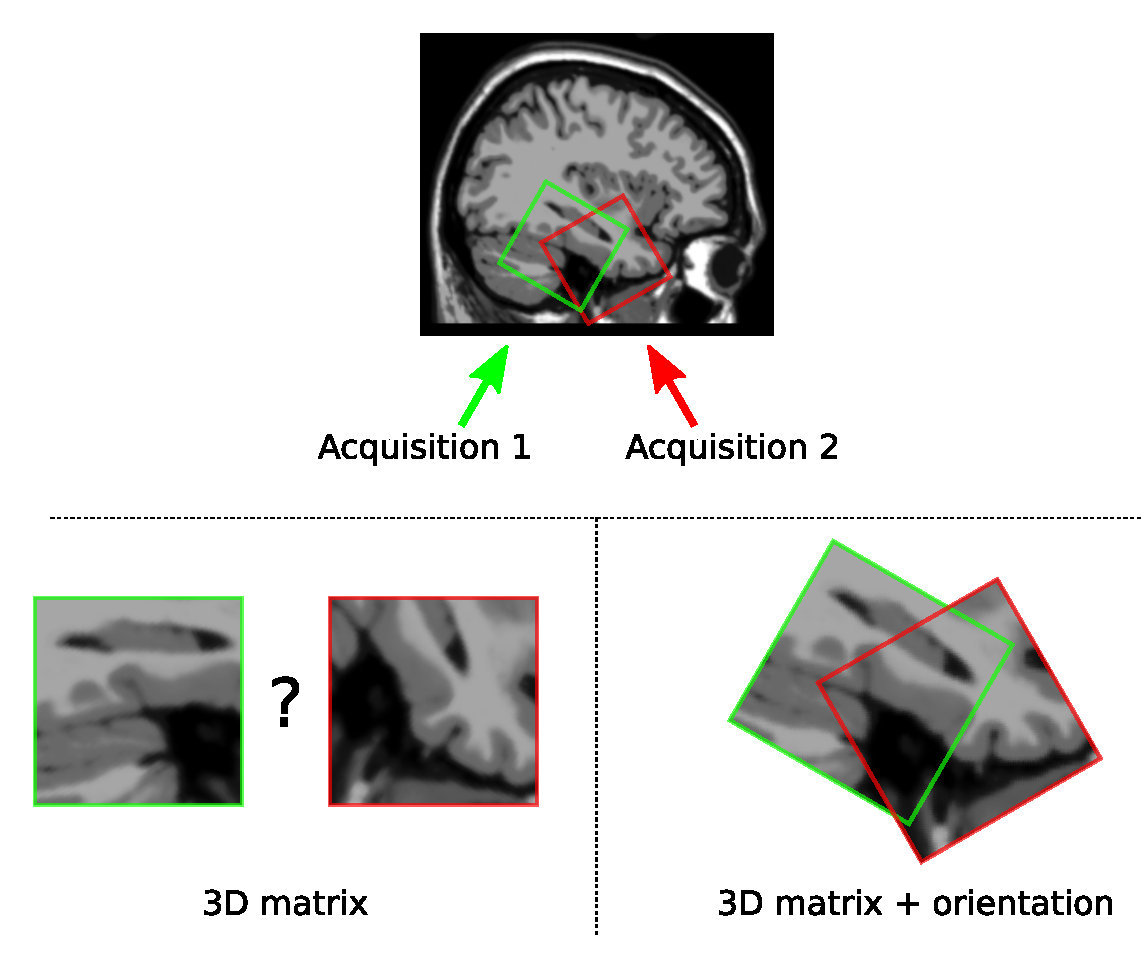
\includegraphics[width=0.5\linewidth]{orientation.pdf} 
\caption{Acquisition of two images at different angles of incidence. Without position information (bottom left picture), the two acquisition cannot be superimposed and are difficult to compare. With the position information (bottom right picture), the two acquisition are trivially superimposed.}
\label{fig:position}
\end{figure}


\section{Coordinate systems}
\label{sec:image:systems}


Let $I$ be a 3D image. If we consider $I$ as an array in a 3-dimensional space, the element of the array in voxel coordinates can be accessed by $I(i,j,k)$ where $i$, $j$, and $k$ are natural numbers including $0$. Given the voxel coordinates $(i,j,k)$, how to project these coordinates into the world coordinates, and conversely? In this section, we answer this simple but essential question.


%----------------------------------------------------------------------------------------------------
\subsection{Projection of coordinates}
\label{subsec:images:systems:projection}

Given a 3D image $I$, let $A$ be a matrix 3$\times$3 and $T$ be a vector in the 3-dimensional space. $A$ and $T$ contain the necessary information to position the 3D array (grid) into the world coordinates. Let $(i,j,k)$ be voxel coordinates, the corresponding position in the word coordinates is given by:

\begin{equation}
\begin{bmatrix} x \\ y \\ z \end{bmatrix}
=
A.
\begin{bmatrix} i \\ j \\ k \end{bmatrix}
+ T
\label{eq:projection1}
\end{equation}

where

\begin{equation}
T = \begin{bmatrix} t_x \\ t_y \\ t_z \end{bmatrix}
\end{equation}

and

\begin{equation}
A =
\begin{bmatrix}
a_{1,1} & a_{1,2} & a_{1,1} \\
a_{2,1} & a_{2,2} & a_{2,1} \\
a_{3,1} & a_{3,2} & a_{3,1}
\end{bmatrix}.
\end{equation}


$T$ contains the position of the image origin in world coordinates while $A$ contains information on voxel size and image orientation. This projection from the voxel to the world coordinates usually uses a 4$\times$4 matrix in homogeneous coordinates:

\begin{equation}
\begin{bmatrix} x \\ y \\ z \\ 1 \end{bmatrix}
=
M.
\begin{bmatrix} i \\ j \\ k \\ 1 \end{bmatrix}
\label{eq:projection2}
\end{equation}

where

\begin{equation}
M =
\begin{bmatrix}
a_{1,1} & a_{1,2} & a_{1,1} & t_x \\
a_{2,1} & a_{2,2} & a_{2,1} & t_y \\
a_{3,1} & a_{3,2} & a_{3,1} & t_z \\
0 & 0 & 0 & 1
\end{bmatrix}
\end{equation}

Both projections (\ref{eq:projection1}) and (\ref{eq:projection2}) are identical and we will use in this report one or the other.
\\

 
Let us now consider $(x,y,z)$ a 3D position in the world coordinates. The projection of this point into the voxel coordinates $(i,j,k)$ is given by:

\begin{equation}
\begin{bmatrix} i \\ j \\ k \end{bmatrix}
=
A^{-1}.
\left(
\begin{bmatrix} x \\ y \\ z \end{bmatrix}
- T
\right)
\end{equation}

One should note that $i$, $j$, $k$ value are not necessarily integer. If so, the value $I(i,j,k)$ is then obtained by image interpolation. This notion will be discussed on section~\ref{sec:image:interpolation}. If we consider a 4$\times$4 matrix in homogeneous coordinates, the projection from world to voxel coordinates is given by:

\begin{equation}
\begin{bmatrix} i \\ j \\ k \\ 1 \end{bmatrix}
=
M^{-1}.
\begin{bmatrix} x \\ y \\ z \\ 1 \end{bmatrix}
\end{equation}


For clarity purpose, we may write in this report $I(x,y,z)$ (or simply $I(\mathbf{x})$ where $\mathbf{x}=(x,y,z)$) where $(x,y,z)$ are world coordinates. The notation $I(x,y,z)$ is abusing and we define  

\begin{equation}
I(x,y,z) \triangleq I(i,j,k)
\end{equation}

where $(i,j,k)$ is the projection of $(x,y,z)$ into the voxel coordinates. The nature of the coordinates will indicate which notation is used.



%----------------------------------------------------------------------------------------------------
\subsection{Positioning information in \texttt{itk::Image} object}
\label{subsec:images:position:itk}


The ITK image format (\texttt{itk::Image}) contains the three following information to position any image into the world coordinated:

\begin{itemize}
\item position of image origin
\item voxel size
\item image orientation (called \textit{direction cosine})
\end{itemize}

These information are respectively retrieved using functions \texttt{GetOrigin()}, \texttt{GetSpacing()}, and \texttt{GetDirection()}, functions inherited from objet \texttt{itk::ImageBase}. Image origin and voxel size (respectively noted $T$ and $S$) are stored as vector in a 3-dimensional space (\texttt{itk::Vector}):

\begin{equation}
T = \begin{bmatrix} t_x \\ t_y \\ t_z \end{bmatrix}
\end{equation}

\begin{equation}
S = \begin{bmatrix} s_x \\ s_y \\ s_z \end{bmatrix}
\end{equation}

Image orientation is stored as a 3$\times$3 matrix (\texttt{itk::Matrix}) noted here $D$:

\begin{equation}
D =
\begin{bmatrix}
d_{1,1} & d_{1,2} & d_{1,1} \\
d_{2,1} & d_{2,2} & d_{2,1} \\
d_{3,1} & d_{3,2} & d_{3,1}
\end{bmatrix}
\end{equation}

To be consistent with notations introduction in Eq.~(\ref{eq:projection1}), we define the 3$\times$3 matrix $A$ as follows:

\begin{equation}
A=D.S_{diag}
\end{equation}

where 

\begin{equation}
S_{diag} =
\begin{bmatrix}
s_x & 0 & 0 \\
0 & s_y & 0 \\
0 & 0 & s_z
\end{bmatrix}.
\end{equation}

Vector $T$ and matrix $A$ allow to project voxel to world coordinates, and conversely (see Eq.~(\ref{eq:projection1})).



%----------------------------------------------------------------------------------------------------
\subsection{Positioning information in Inrimages image format}

The Inrimage format contains all the information needed to position any image into the world coordinated:

\begin{itemize}
\item $TX$, $TY$, and $TZ$ is the position of the image origin (resp. along the X-, Y-, and Z-axes),
\item $VX$, $VY$, and $VZ$ give the voxel size,
\item $RX$, $RY$, and $RZ$ correspond to the image orientation.
\end{itemize}

As in section~\ref{subsec:images:position:itk}, we define the vector $T$ and $S$ as follows:

\begin{equation}
T = \begin{bmatrix} TX \\ TY \\ TZ \end{bmatrix}
\end{equation}

\begin{equation}
S = \begin{bmatrix} VX \\ VY \\ VZ \end{bmatrix}
\end{equation}

The image orientation (noted $D$ in section~\ref{subsec:images:position:itk}) is computed from values RX, RY et RZ. First, we define the vector $R$ as follows:

\begin{equation}
R = \begin{bmatrix} RX \\ RY \\ RZ \end{bmatrix}.
\end{equation}

Then, let $N$ be the normalized vector

\begin{equation}
N = \begin{bmatrix} n_x \\ n_y \\ n_z \end{bmatrix}
= \begin{bmatrix} RX/\phi \\ RY/\phi \\ RZ/\phi \end{bmatrix}
\end{equation}

where $\phi$ is the Euclidean norm of R. Finally, the orientation matrix $D$ is given by:

\begin{equation}
D =
cos \phi
\begin{bmatrix}
1 & 0 & 0 \\
0 & 1 & 0 \\
0 & 0 & 1
\end{bmatrix}
+ (1 - cos \phi)
\begin{bmatrix}
n_x^2 & n_x n_y & n_x n_z \\
n_x n_y & n_y^2 & n_y n_z \\
n_x n_z & n_x n_y & n_z^2
\end{bmatrix}
+ sin \phi
\begin{bmatrix}
0 & -n_z & n_y \\
n_z & 0 & -n_x \\
-n_y & n_x & 0
\end{bmatrix}
\end{equation}

As in section~\ref{subsec:images:position:itk}, the 3$\times$3 matrix $A$ defined in Eq.~(\ref{eq:projection1}) an necessary to project voxel coordinates into the world coordinates is given by:

\begin{equation}
A=D.S_{diag}
\end{equation}


\section{Image interpolation}
\label{sec:image:interpolation}



Let $I$ be an image of size $[w,h,d]$ (resp. width, height, and depth). As explained in section~\ref{sec:image:systems}, the image is the representation (discretization) of a volume in the world coordinate system.
Let $\mathbf{x}=(x,y,z)$ be the coordinates of a point in the world coordinate such that $\mathbf{x}$ is included into the acquired volume. In other words, if $\mathbf{i}=(i,j,k)$ is the projection of $\mathbf{x}$ in the voxel coordinates (see section~\ref{subsec:images:systems:projection}), we have:
%
\begin{equation}
\mathbf{i} \in [0,w-1]\times[0,h-1]\times[0,d-1]
\end{equation}
%
If $\mathbf{x}$ is randomly drawn in the image volume, the coordinates $(i,j,k)$ are probably not integer and $I(i,j,k)$ is not defined. The image interpolation consists in computing the image value at any index $(i,j,k)$ -- integer or not -- usually using the local neighborhood of $(i,j,k)$. Many algorithms have been proposed in the literature and we present in this section a very short list of the most classical interpolation methods. In the case of $(i,j,k)$ are out of the image bound is usually treated differently from the case where $(i,j,k)$ are in the image bound. This case will not be treated below.



%----------------------------------------------------------------------------------------------------
\subsection{Nearest neighbor interpolation}

The interpolation to the nearest neighbor is the fastest and the simplest interpolation method.
Given $(i,j,k)$ a non integer voxel coordinates, the image value at $(i,j,k)$ is given by
%
\begin{equation}
I(i,j,k) \triangleq I( \underline{i}, \underline{j}, \underline{k} )
\end{equation}
%
where $( \underline{i}, \underline{j}, \underline{k} )$ are respectively the round to the nearest integer of $(i,j,k)$.
One particularity of the nearest neighbor interpolation -- which can be considered as an issue -- is that the image value is constant on an elementary volume centered around the integer coordinates ; if $(i,j,k)$ are here integer coordinates, we have
%
\begin{equation}
I(i+\epsilon_1,j+\epsilon_2,k+\epsilon_3) = I(i,j,k)
\end{equation}
%
for $\epsilon_{i=\{1,3\}} \in (-0.5,0.5)$. Note that in the case where $|\epsilon_{i=\{1,3\}}| = 0.5$, the selected nearest neighbor depends on the implementation of the rounding procedure. Usually, the nearest neighbor of $i+0.5$ is $i+1$, and, as a consequence, the nearest neighbor of $i-0.5$ is $i$.



%----------------------------------------------------------------------------------------------------
\subsection{Linear interpolation}

Given $a$ a real number, we define $\lceil a \rceil$ and $\lfloor a \rfloor$ respectively as the round up (towards plus infinity) andthe round down (towards minus infinity) of $a$. Let $(i,j,k)$ be non integer voxel coordinates, and let $\alpha, \beta, \gamma$ be the weights defined as:
%
\begin{align}
\alpha= & \lceil i \rceil - i \\
\beta=  & \lceil j \rceil - j \\
\gamma= & \lceil k \rceil - k \\
\end{align}
%
The coordinates $(i,j,k)$ belongs by definition to the intervale $[ \lfloor i \rfloor , \lceil i \rceil]\times$ $[ \lfloor j \rfloor , \lceil i \rceil]\times$ $[ \lfloor i \rfloor , \lceil k \rceil]$. This intervale corresponds to a cuboid in the world coordinates where each one of its height corners is an element of the grid. The tri-linear interpolation uses the image values at these corners, the value at a given corner being simply weighted by a function of the distance between of the corner and the index $(i,j,k)$:
%
\begin{align}
\nonumber I(i,j,k) & \triangleq I(\lfloor i \rfloor, \lfloor j \rfloor, \lfloor k \rfloor) * \alpha \beta \gamma\\
\nonumber          & + I(\lceil  i \rceil , \lfloor j \rfloor, \lfloor k \rfloor) * (1-\alpha)\beta\gamma\\
\nonumber          & + I(\lfloor i \rfloor, \lceil  j \rceil , \lfloor k \rfloor) * \alpha (1-\beta) \gamma\\
\nonumber          & + I(\lfloor i \rfloor, \lfloor j \rfloor, \lceil  k \rceil ) * \alpha\beta(1-\gamma)\\
\nonumber          & + I(\lceil  i \rceil , \lceil  j \rceil , \lfloor k \rfloor) * (1-\alpha) (1-\beta) \gamma\\
\nonumber          & + I(\lceil  i \rceil , \lfloor j \rfloor, \lceil  k \rceil ) * (1-\alpha)\beta(1-\gamma)\\
\nonumber          & + I(\lfloor i \rfloor, \lceil  j \rceil , \lceil  k \rceil ) * \alpha(1-\beta)(1-\gamma)\\
                   & + I(\lceil  i \rceil , \lceil  j \rceil , \lceil  k \rceil ) * (1-\alpha)(1-\beta)(1-\gamma                   \label{eq:images:interpolation:linear}
\end{align}
%
One interesting property of this interpolation method is that, contrary to the nearest neighbor interpolation method, there are no discontinuity in terms of values in the image volume. Moreover, the formula (\ref{eq:images:interpolation:linear}) is still valid even if $(i,j,k)$ are valid integer coordinates.
\\
However, if the initial image was coded for instance on integer (\textit{e.g.} \texttt{short}), the interpolation introduce non integer value that may be not adapted for some processing or visualization. In this case, the nearest neighbor interpolation is more adapted.




%----------------------------------------------------------------------------------------------------
%\subsection{Interpolation en volumes partiels}
